

\tikzset{every picture/.style={line width=0.75pt}} %set default line width to 0.75pt        

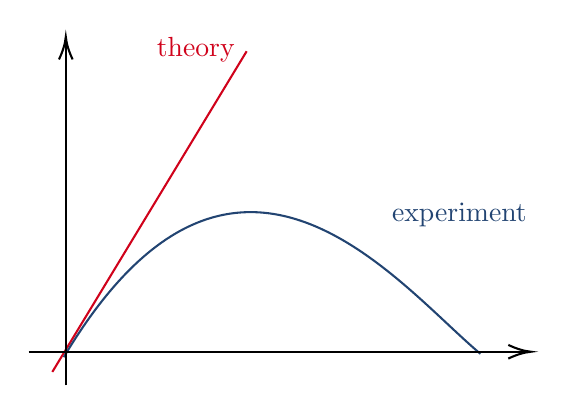
\begin{tikzpicture}[x=0.75pt,y=0.75pt,yscale=-1,xscale=1]
%uncomment if require: \path (0,300); %set diagram left start at 0, and has height of 300

%Straight Lines [id:da44773090746859867] 
\draw [color={rgb, 255:red, 208; green, 2; blue, 27 }  ,draw opacity=1 ]   (100.87,233.5) -- (194.5,79) ;
%Curve Lines [id:da7265875796819894] 
\draw [color={rgb, 255:red, 34; green, 68; blue, 114 }  ,draw opacity=1 ]   (106.37,226.38) .. controls (188.5,89) and (266.53,190.65) .. (307.14,224.76) ;
%Straight Lines [id:da8045363903004159] 
\draw    (89.5,223.76) -- (329.5,223.76) ;
\draw [shift={(331.5,223.76)}, rotate = 180] [color={rgb, 255:red, 0; green, 0; blue, 0 }  ][line width=0.75]    (10.93,-3.29) .. controls (6.95,-1.4) and (3.31,-0.3) .. (0,0) .. controls (3.31,0.3) and (6.95,1.4) .. (10.93,3.29)   ;
%Straight Lines [id:da5761614694400692] 
\draw    (107.37,240) -- (107.37,74) ;
\draw [shift={(107.37,72)}, rotate = 450] [color={rgb, 255:red, 0; green, 0; blue, 0 }  ][line width=0.75]    (10.93,-3.29) .. controls (6.95,-1.4) and (3.31,-0.3) .. (0,0) .. controls (3.31,0.3) and (6.95,1.4) .. (10.93,3.29)   ;

% Text Node
\draw (170,78) node  [color={rgb, 255:red, 208; green, 2; blue, 27 }  ,opacity=1 ] [align=left] {theory};
% Text Node
\draw (297,158) node  [color={rgb, 255:red, 34; green, 68; blue, 114 }  ,opacity=1 ] [align=left] {experiment};


\end{tikzpicture}